

\documentclass[a4paper, 8pt]{article}
\usepackage{graphicx} % Required for inserting images
\usepackage{amsmath}
\usepackage{amssymb}
\usepackage{geometry}
\usepackage{enumitem}
\geometry{margin=1in}
\usepackage{pgfplots}
\pgfplotsset{compat=1.18}
\usepackage{ragged2e}
\usepackage{etoolbox}

\title{PSP Coursework}
\author{Timothy Chung}
\date{November 2024}

\begin{document}

\maketitle

\section*{Solutions}
% Apply \RaggedRight globally
\RaggedRight % Apply it to regular text



\subsection*{Q1: Random Variables}

\begin{enumerate}[label=\alph*)]
    \item \textbf{We place uniformly at random $n = 200$ points in the unit interval $[0, 1]$. Denote by the random variable $X$ the distance between $0$ and the first random point on the left.}

          \begin{enumerate}[label=\roman*)]
              \item \textbf{Find the probability distribution function $F_X(x)$.}

                    Note: we use $F_X(x)$ to refer to the PDF and not the CDF in this question only. Since $n$ points are placed uniformly on $[0, 1]$, the probability that no point lies within the interval $[0, x]$ with $x \in [0, 1]$ is given by:
                    \begin{align*}
                        F_X(x) & = \text{Probability of no point in } [0, x] \\
                               & = (1 - x)^n                                 \\
                               & = (1-x)^{200}
                    \end{align*}
                    Where $ 0 \leq x \leq 1$. Here, points are placed such that they are i.i.d..

              \item \textbf{Derive the limit as $n \to \infty$ and comment on your expression.}

                    We revise our notation to parametrise the number of samples drawn.

                    \[
                        F_X(x;n) = (1 - x)^n
                    \]

                    For large $n$, we take the limit as $n \to \infty$, observe that for any fixed $x \in (0, 1]$:
                    \[
                        F_X(x;n) \to 0
                    \]
                    However, for $x = 0$:
                    \[
                        \lim_{n \to \infty }F_X(0;n) = \lim_{n \to \infty }(1 - 0)^n = 1
                    \]


                    This is because for the uniform distribution, the probability of selecting a single point ($x=0$) is always zero. So we are sure with absolute certainty that there will be no points directly on $0$. In conclusion, when $n \to \infty$:

                    \[
                        F_X(x) =
                        \begin{cases}
                            1 & \text{if } x = 0        \\
                            0 & \text{if } x \in (0, 1] \\
                            0 & \text{otherwise}
                        \end{cases}
                    \]
          \end{enumerate}
    \item \textbf{The random variable $X$ is uniform in the interval $(0, 1)$. Find the density function of the random variable $Y = -\ln X$.}

          Since $X$ is uniform on $(0, 1)$, the probability density function (PDF) of $X$ is:
          \[
              f_X(x) =
              \begin{cases}
                  1, & 0 < x < 1        \\
                  0, & \text{otherwise}
              \end{cases}
          \]
          The transformation $Y = -\ln X$ implies that $X = e^{-Y}$. Taking the derivative:
          \[
              \frac{dX}{dY} = -e^{-Y}.
          \]
          The support of $Y$ is derived as follows:
          \[
              X \in (0, 1) \implies -\ln X \in (0, \infty) \implies Y \in (0, \infty)
          \]
          Using the change of variables formula:
          \[
              f_Y(y) = f_X(x) \left| \frac{dX}{dY} \right|, \quad x = e^{-y}, \quad \left| \frac{dX}{dY} \right| = e^{-y}
          \]
          Substituting \( f_X(x) = 1 \) for \( x \in (0, 1) \), we get:
          \[
              f_Y(y) = e^{-y}, \quad y > 0
          \]
          Therefore, the PDF of $Y$ is:
          \[
              f_Y(y) =
              \begin{cases}
                  e^{-y} & y > 0            \\
                  0      & \text{otherwise}
              \end{cases}
          \]

          \begin{figure}[h!]
              \centering
              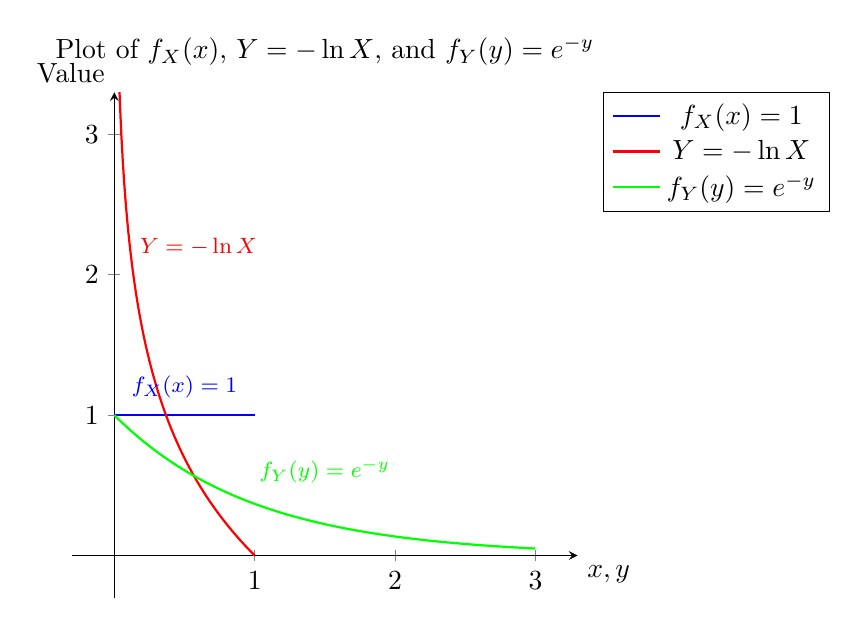
\begin{tikzpicture}
                  \begin{axis}[
                          axis lines=middle,
                          xlabel={$x, y$},
                          ylabel={Value},
                          ymin=0, ymax=3,
                          xmin=0, xmax=3,
                          xtick={0, 1,2,3},
                          ytick={0, 1, 2, 3},
                          xlabel style={below right},
                          ylabel style={above left},
                          legend style={at={(1.05,1)}, anchor=north west},
                          title={Plot of $f_X(x)$, $Y = -\ln X$, and $f_Y(y) = e^{-y}$},
                          height=8cm,
                          width=8cm,
                          enlargelimits=true,
                      ]
                      % Plot f_X(x): Uniform distribution on (0, 1)
                      \addplot[thick, blue, domain=0:1] {1};
                      \addlegendentry{$f_X(x) = 1$}

                      % Plot Y = -ln(x): Transformation of X
                      \addplot[thick, red, domain=0.01:1, samples=100] {-ln(x)};
                      \addlegendentry{$Y = -\ln X$}

                      % Plot f_Y(y) = e^{-y}: PDF of Y
                      \addplot[thick, green, domain=0:3, samples=100] {exp(-x)};
                      \addlegendentry{$f_Y(y) = e^{-y}$}

                      % Add annotations
                      \node[blue] at (axis cs:0.5, 1.2) {\footnotesize $f_X(x) = 1$};
                      \node[red] at (axis cs:0.6, 2.2) {\footnotesize $Y = -\ln X$};
                      \node[green] at (axis cs:1.5, 0.6) {\footnotesize $f_Y(y) = e^{-y}$};
                  \end{axis}
              \end{tikzpicture}
              \caption{Combined plot of $f_X(x)$, $Y = -\ln X$, and $f_Y(y) = e^{-y}$. Note that $f_Y(y)$ is the reflection of $Y$ over the line $y=x$}.
          \end{figure}


    \item \textbf{$X$ and $Y$ are independent, identically distributed (i.i.d.) random variables with common PDF $f_X(x) = e^{-x}, \, x > 0$. Find the PDFs of the following random variables:}

          \begin{enumerate}[label=\roman*)]
              \item \textbf{$Z = X \cdot Y$.}

                    Because $X$ and $Y$ are independent, the PDF of $Z = X \cdot Y$ is just the product of both PDFs. The joint distribution of $X$ and $Y$ is:
                    \[
                        f_{X,Y}(x, y) = f_X(x) f_Y(y) = e^{-x} e^{-y}, \quad x, y > 0.
                    \]
                    For $Z = X \cdot Y$, we transform the PDF using the Jacobian Determinant for 1D transformation:

                    % The random variable \( Z = X \cdot Y \) can be expressed using the joint PDF of \( X \) and \( Y \), where \( Y = Z / X \). The PDF of \( Z \) is obtained as:

                    \[
                        f_Z(z) = \int_0^\infty f_{X,Y}\left(x, \frac{z}{x}\right) \left|\frac{\partial y}{\partial z}\right| dx,
                    \]

                    where \( y = \frac{z}{x} \). The Jacobian determinant accounts for the change of variables:

                    \[
                        \frac{\partial y}{\partial z} = \frac{1}{x}.
                    \]

                    Thus, the absolute value of the Jacobian determinant is:

                    \[
                        \left|\frac{\partial y}{\partial z}\right| = \frac{1}{x}.
                    \]

                    Substituting this into the integral, we have:

                    \[
                        f_Z(z) = \int_0^\infty f_{X,Y}\left(x, \frac{z}{x}\right) \frac{1}{x} dx,
                    \]

                    where \( f_{X,Y}(x, y) = f_X(x) f_Y(y) = e^{-x} e^{-y}, \, x, y > 0 \).


                    \[
                        f_Z(z) = \int_0^\infty f_{X,Y}(x, z/x) \frac{1}{x} \, dx.
                    \]
                    Substituting \( f_{X,Y}(x, z/x) = e^{-x} e^{-z/x} / x \), the integral becomes:
                    \[
                        f_Z(z) = \int_0^\infty e^{-x} e^{-z/x} \frac{1}{x} \, dx, \quad z > 0.
                    \]
                    Solving this integral (using substitution or standard tables):
                    \[
                        f_Z(z) = 2 K_0(2 \sqrt{z}), \quad z > 0,
                    \]
                    where \( K_0 \) is the modified Bessel function of the second kind.

              \item \textbf{$Z = \frac{X}{Y}$.}
                    The CDF of \( Z \) is defined as:

                    \[
                        F_Z(z) = P\left( \dfrac{X}{Y} \leq z \right) = P(X \leq zY).
                    \]

                    Since \( X \) and \( Y \) are independent, we can express this probability as an integral over the PDF of \( Y \):

                    \[
                        F_Z(z) = \int_{0}^{\infty} P(X \leq zy) f_Y(y) \, dy.
                    \]

                    Given that \( X \) is exponential, the probability \( P(X \leq zy) \) becomes:

                    \[
                        P(X \leq zy) = \int_{0}^{zy} e^{-x} \, dx = 1 - e^{-zy}.
                    \]

                    Substituting back into the expression for \( F_Z(z) \):

                    \[
                        F_Z(z) = \int_{0}^{\infty} \left(1 - e^{-zy}\right) e^{-y} \, dy.
                    \]


                    Split the integral into two parts:

                    \[
                        F_Z(z) = \int_{0}^{\infty} e^{-y} \, dy - \int_{0}^{\infty} e^{-y} e^{-zy} \, dy = I_1 - I_2.
                    \]

                    Compute \( I_1 \) and \( I_2 \):

                    \begin{enumerate}[label=(\alph*)]
                        \item \textbf{First Integral \( I_1 \):}

                              \[
                                  I_1 = \int_{0}^{\infty} e^{-y} \, dy = \left[ -e^{-y} \right]_0^\infty = 0 - (-1) = 1.
                              \]

                        \item \textbf{Second Integral \( I_2 \):}

                              \[
                                  I_2 = \int_{0}^{\infty} e^{-y(1 + z)} \, dy = \frac{1}{1 + z}.
                              \]

                              This follows from the standard integral of the exponential function:

                              \[
                                  \int_{0}^{\infty} e^{-k y} \, dy = \frac{1}{k}, \quad \text{for } k > 0.
                              \]
                    \end{enumerate}

                    Therefore, the CDF \( F_Z(z) \) becomes:

                    \[
                        F_Z(z) = 1 - \frac{1}{1 + z} = \frac{z}{1 + z}, \quad z \geq 0.
                    \]

              \item \textbf{Differentiate to Find the PDF \( f_Z(z) \):}

                    The PDF is the derivative of the CDF:

                    \[
                        f_Z(z) = \frac{d}{dz} F_Z(z) = \frac{d}{dz} \left( \frac{z}{1 + z} \right).
                    \]

                    Compute the derivative using the quotient rule:

                    \[
                        f_Z(z) = \frac{(1 + z)(1) - z(1)}{(1 + z)^2} = \frac{1}{(1 + z)^2}, \quad z \geq 0.
                    \]

                    Thus, the PDF of \( Z \) is:

                    \[
                        f_Z(z) = \frac{1}{(1 + z)^2}, \quad z \geq 0.
                    \]

              \item \textbf{$Z = \max(X, Y)$.}

                    The CDF of $Z$ is:
                    \[
                        F_Z(z) = P(\max(X, Y) \leq z) = P(X \leq z \text{ and } Y \leq z) = P(X \leq z) P(Y \leq z),
                    \]
                    since $X$ and $Y$ are independent. Substituting the CDFs of $X$ and $Y$:
                    \[
                        F_Z(z) = (1 - e^{-z})^2, \quad z > 0.
                    \]
                    Differentiating to get the PDF:
                    \[
                        f_Z(z) = \frac{d}{dz} F_Z(z) = 2(1 - e^{-z})e^{-z}, \quad z > 0.
                    \]

          \end{enumerate}
\end{enumerate}

\end{document}
